\section{Analysis - Total Interaction Cross Section $^{12}$C + $^{12}$C - $^{12}$C + $^{12}$C}
This chapter will go through the  analysis step by step from the unpacking stage to the final measurement of the total reaction cross section. It will start by a short overview of the transmission method used for the cross section measurements. The next step is  the selection of clean incoming $^{12}$C isotopes. Following the identification of the carbon isotopes after the target - for the measurement of the charge changing cross section - and as final step the reaction cross section measurement. \newline
All relevant detector related geometrical and efficiency corrections will be adressed and their influence to the final result and its uncertainty will be discussed.
\subsection{Cross Section Measurement via Transmission Method}
In its most generic form cross sections give a measure of the probability that a specific reaction will take place when two or more particles collide. The cross sections  measured in scattering exepriments, as well as the energy and angular distribution of the reaction products, provide information about the dynamics of the interaction between the projectile and the target particle, i.e., about the shape of the interaction potential and the coupling strength.\newline
The cross section $\sigma$ can be derived by looking at the relation between the number of incoming particles (N$_{1}$) and unreacted particles after collision ($N_{2}$). For an experiment with fixed target with thickness $z$ and volumetric number density $n$ the number of reacted particles in the infinitesimal thin target layer $dz$ can be expressed as:
\begin{equation}
\frac{dN_{2}}{dz} = -n \sigma N_{2}
\end{equation}
Solving this differential equation for $N_{2}$ (with the condition $N_{2}$ = $N_{1}$ for $z=0$) discloses an exponential relation:
\begin{equation}
N_{2} = N_{1}e^{-n\sigma z}
\label{eq:cross_sec}
\end{equation} 
Where $n z$ can be summarized as $N_t$, the total number of scattering centers per unit area. The relation $(N_{2}/N_{1})$, number of unreacted particles after collision versus number of incoming particles, is often called survival probability. For an idealistic experimental setup with full detector efficiency and no interactions in the setup material the cross section could simply be deduced from equation \ref{eq:cross_sec}. To account for reactions of the projectile that occur within the setup material and first order detector specific distortions of output signals the survival probabiltiy $(N_{2}/N_{1})$ has to be divided by $(N_{2}^E/N_{1}^E)$, where $N_{1}^E$ is the number of incoming particles and $N_{2}^E$ the number of unreacted particles after collision for an empty run respectively. The factor $(N_{2}^E/N_{1}^E)$ can also be seen as an overall-experiment specific efficiency. The final formula for the cross section for a so called transmission measurement is:
\begin{equation}
\sigma = -\frac{1}{N_t} ln(\frac{1}{\epsilon_{setup}} \frac{N_2}{N_1}),\quad with \quad  \epsilon_{setup} = \frac{N_{2}^E}{N_{1}^E}
\label{eq:corr_cross}
\end{equation}
From the above formula \ref{eq:corr_cross} it is evident that for cross section measurements with the transmission method three types of observables have to be measured:\newline
\begin{enumerate}
\item[$\blacksquare$] \textbf{Number of scattering centers $N_t$}\newline
The number of scattering centers per unit area of the target is a target specific number. It depends from the target thickness and and its density. The values herefore are taken from \cite{ponnath2023precise}\footnote{For the purpose of this work the target thicknesses were remeasured at GSI with a chromatic sensor giving 2D depth profiles of each target.}. 
\item[$\blacksquare$] \textbf{Number of incoming projectiles ($^{12}$C) $N_1$}
For the measurement only events with well identified incoming $^{12}$C projectiles are chosen. Herefore strict cuts on the detectors upstream the target are set. This strict (upstream) event selection makes sure that we only consider events with single $^{12}$C ...See more in section \ref{subsec:event-sel}.  %TODO finish this sencence 
\item[$\blacksquare$] \textbf{Number of unreacted projectiles ($^{12}$C) $N_2$ after the target}
Detectors downstream the target are used to count the number of unreacted projectiles $^{12}$C. To reduce detector specific influences which could distort the result it is advisable to use only as few as requirable detectors for the clear identification of unreacted projectiles. Moreover detector specific efficiencies which only depend of the beam energy are cancelled out by including both empty and target runs in the cross section calculation, see equation\ref{eq:corr_cross}. For all downstream detectors used in this analyisis it is critical to limit any selection cuts to what is necessary and if necessary systematically check their effects on the counted number $N_2$.
\end{enumerate}
\subsection{Event Selection}\label{subsec:event-sel}
\begin{figure}[htpb]
    \centering
    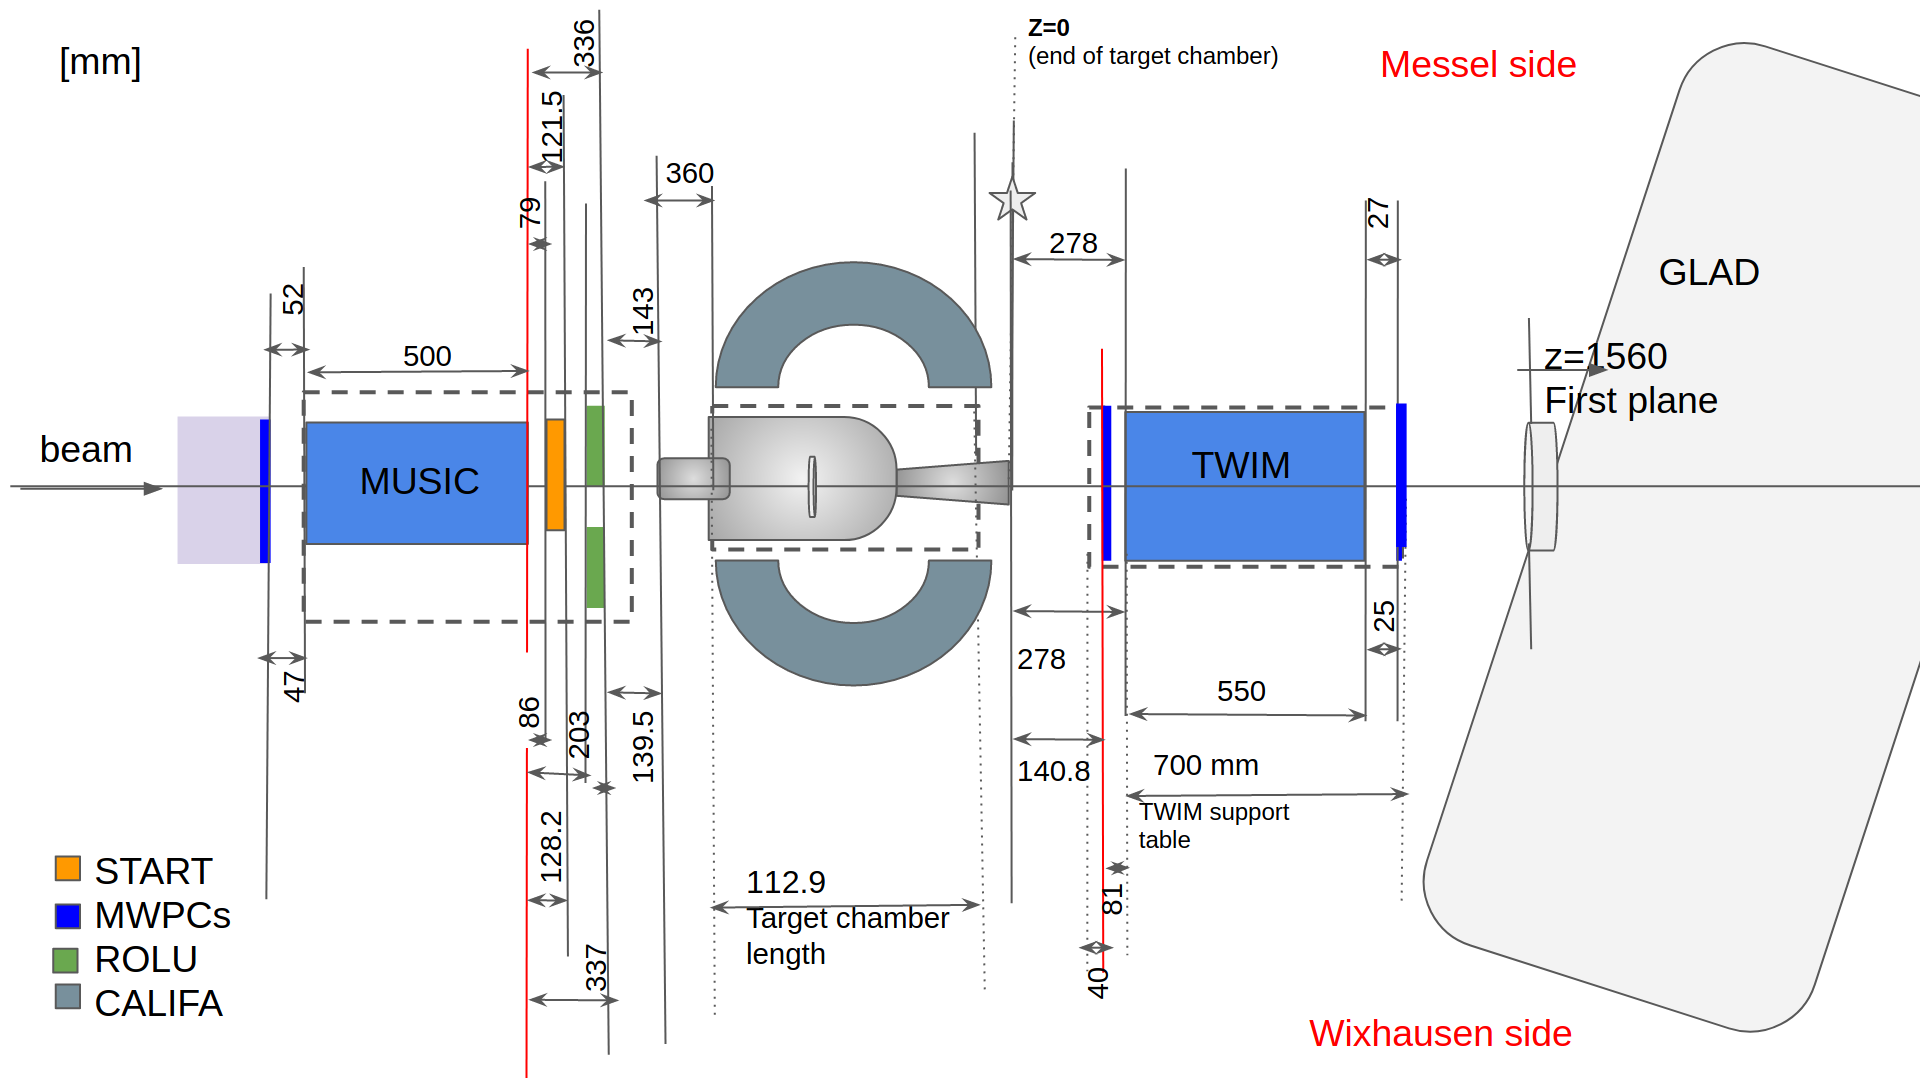
\includegraphics[width=\textwidth,height=6cm,keepaspectratio=true]{Figures/SETUP_around_Target.png}
    \caption{
    R3B Setup for the S444 experiment in the target region. 
    }
    \label{fig:setup_target_region}
\end{figure}

For event selection, all three upstream detectors are utilized: the MWPC0, the R3BMusic Ionization Chamber, and the START detector. To ensure a clean incoming event selection, the following prerequisites must be met:
\begin{enumerate}
\item $^{12}$C identification of incoming projectile by upstream detectors:\newline
\begin{figure}[htpb]
    \centering
    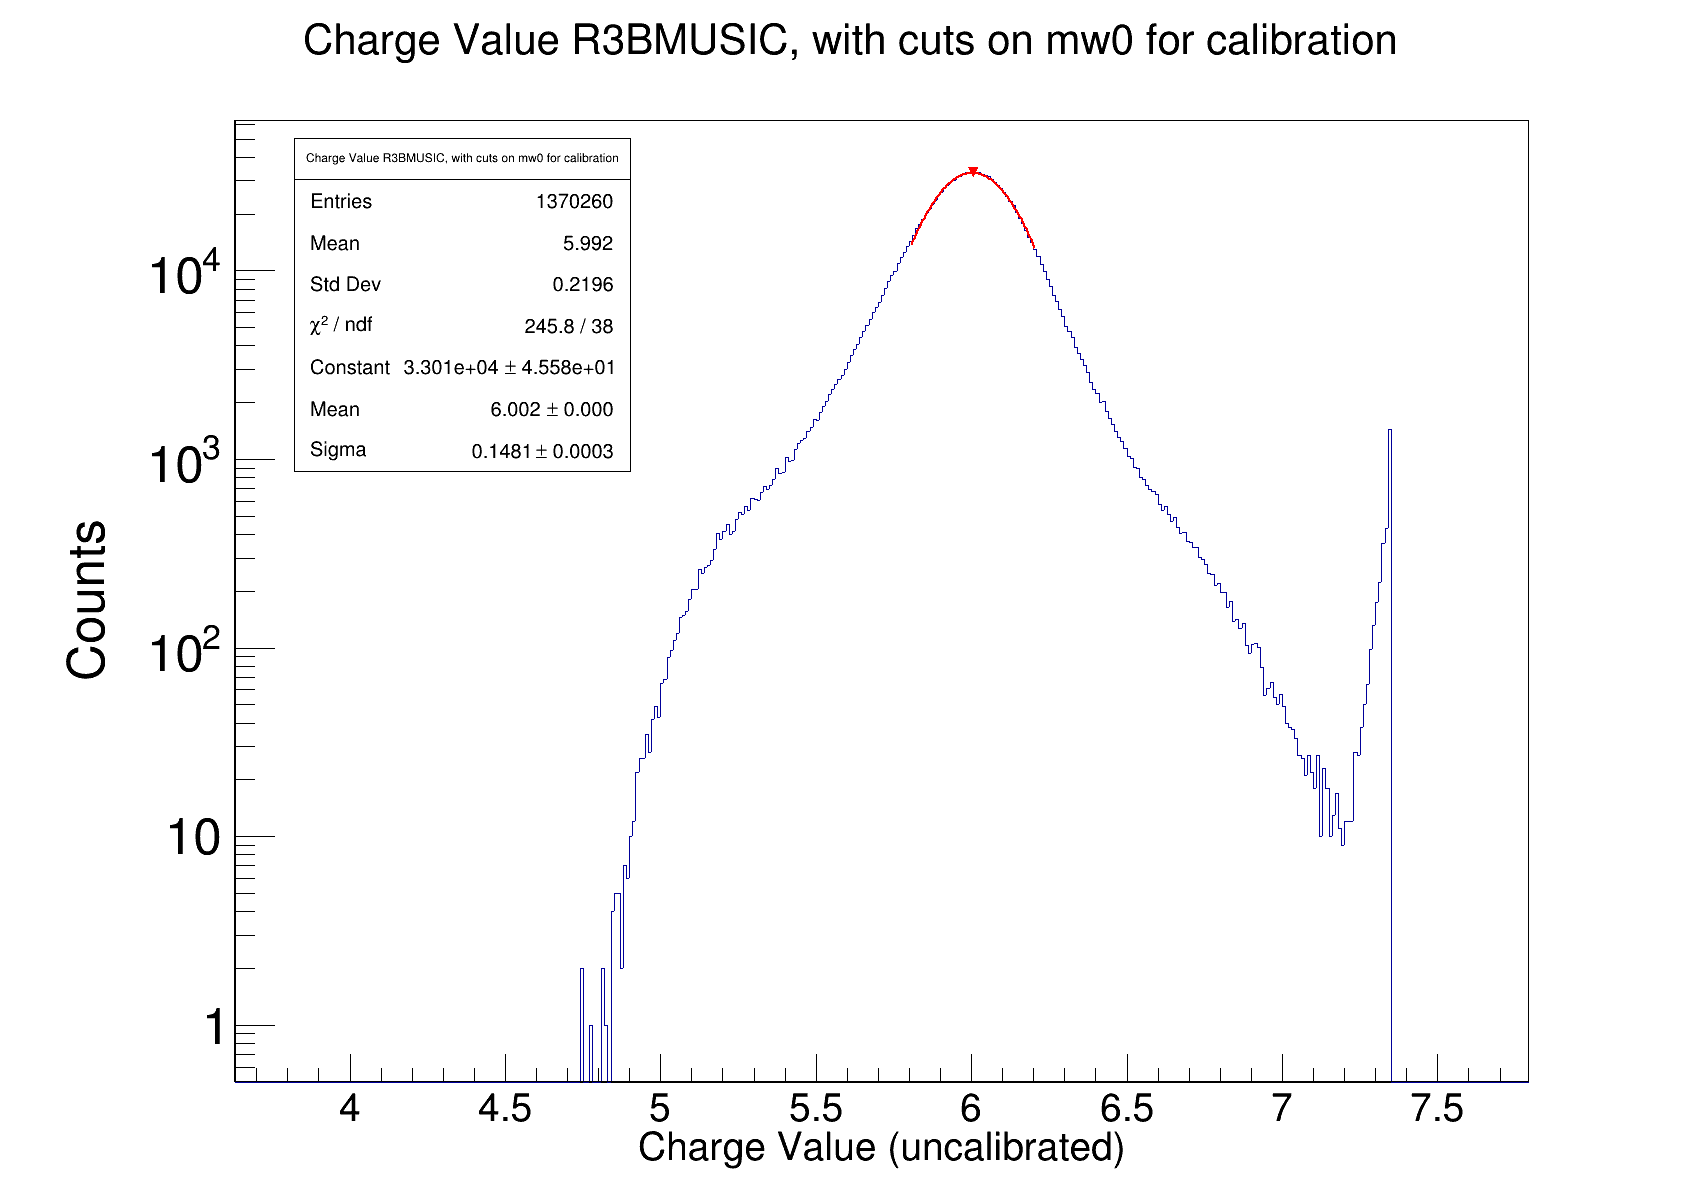
\includegraphics[width=\textwidth,height=6cm,keepaspectratio=true]{Figures/charge_r3bmusic.png}
    \caption{
    Charge distribution on R3BMusic with predefinded calibration parameters with already applied positional cuts on MWPC0 - positioned upstream to the ionisation chamber. 
    }
    \label{fig:r3bmusic_charge}
\end{figure}
In the S444 experiment the incoming beam was directly delivered by the SIS18 ring accelerator, which is operated in ultra-high vacuum the level of pollution is low.(TODO:up to which stage do we have vacuum? Until MW0?)\newline %TODO:up to where is the beam in vacuum?
For the charge identification of the incoming ion the R3BMusic ionisation chamber is used which is positioned directly after the MWPC0 at the beam entrance in Cave C,see figure \ref{fig:setup_target_region}. The R3BMusic detector measures anode-wise the energy loss of the passing-through ion which in the first order is proportional to the square of its charge ($\Delta E \sim Z^{2}$). Herfore the default predefined calibration parameters are used. Figure \ref{fig:r3bmusic_charge} shows the measured charge distribution in R3BMusic. To select $Z = 6$ incoming ions the distibution is fitted. All ions with charge within the $\pm 1 \sigma$ range are accepted.  
\item Pileup rejection and TPat selection:\newline
The overall recoding and merging of the data from various subdetectors is one of the tasks of the Data AcQuisition (DAQ) system. Whether an event is recorded or not depends on the pre-established trigger logic. Various detectors can send out triggers to the main DAQ when certain conditions are given (e.g. CALIFA sends aout a trigger when a hit with more than 20 MeV is recorded). The different triggers are processed by the trigger logic and summarized as a defined trigger pattern, so called TPat, which is stored in a 16-bit mask for each event. Table blabla gives an overview of the trigger logic and the trigger patterns set in the S444 experiment.
\begin{table}[h!]
\centering
\begin{tabular}{||c c c||} 
\hline
Bit Position &TPat Name & Description \\
\hline\hline
0 & Min Bias & Hit in Start detector\\
\hline
\end{tabular}
\end{table}
\item Projectile's focus on the active target region:
\end{enumerate}
\subsection{Charge Changing Cross Section Measurement}
\subsection{Geometric Corrections}
\subsection{Isotope Correction - Total Interaction Cross Section}
\subsection{Fine Tuned Geometric Correction}
\subsection{Results}
\subsection{qfs analyis}
\subsection{reaction cross section Analysis}

